\section{Auswertung}
\label{sec:Auswertung}

% templates

%\begin{table}
%    \centering
%    \caption{.}
%    \label{tab:}
%    \sisetup{table-format = 3.0} 
%    \begin{tblr}{
%        colspec = {S S S},
%        row{1} = {guard, mode = math}
%    }
%        \toprule 
%        x \mathbin{/} \unit{\milli\meter} \\
%        \midrule
%        %data here
%        \bottomrule
%    \end{tblr}
%\end{table}

%\begin{figure}
%    \centering
%    \includegraphics[width =0.48\textwidth]{}
%    \caption{.}
%    \label{fig:}
%\end{figure}

%\begin{wrapfigure}[20]{r}{0.5\textwidth}
%    \begin{center}
%        \includegraphics[width =0.48\textwidth]{figures/}
%        \caption{}
%        \label{fig:}
%    \end{center}
%\end{wrapfigure}
In der Auswertung werden Abweichung mit der Formel
\begin{equation}
    \text{Abweichung} = \frac{\abs{A_\text{theorie} - A_\text{experiment}}}{A_\text{theorie}}
    \label{eq:Abweichung}
\end{equation}
berechnet. 

\subsection{Invertierender Verstärker}
\label{subsec:Auswertung_InvertierenderVerstaerker}

Die Schaltung des invertierenden Verstärkers wurde gemäß \autoref{fig:invertierenderVerstaerker} aufgebaut. 
Für drei verschiedene Kombinationen von Widerständen $R_1$ und $R_2$ wurde die Verstärkung als Funktion der Frequenz gemessen. 
Die verwendeten Werte der Widerstände können dem \autoref{subsec:InvertierenderVerstaerker} entnommen werden.
Aus den gemessenen Ausgangsspannungen wurde die Verstärkung berechnet und in einem doppelt-logarithmischen Bode-Diagramm dargestellt. 
Die experimentellen Daten wurden mit einem Fit an die Übertragungsfunktion eines idealen Tiefpasses
\begin{equation}
    A(f) = 20 \cdot \log_{10} \left( \frac{A_0}{\sqrt{1 + \left( \frac{f}{f_c} \right)^2}} \right)
    \label{eq:lowPassFilter}
\end{equation}
angepasst und in $\unit{dB}$ umgerechnet.

Die Fits sind in \autoref{plt:invertierenderVerstaerker1}, \ref{plt:invertierenderVerstaerker2} und 
\ref{plt:invertierenderVerstaerker3} dargestellt und liefern 

\begin{itemize}
    \item \textbf{Messung 1:} \\
    Verstärkung $A_0 = 96.76$, $f_c = \qty{5.943}{\kilo\hertz}$, erwartete Verstärkung $\frac{R_2}{R_1} = 100$, Abweichung von $\qty{3.24}{\percent}$
    \item \textbf{Messung 2:} \\
    Verstärkung $A_0 = 148.28$, $f_c = \qty{6.923}{\kilo\hertz}$, erwartete Verstärkung $\frac{R_2}{R_1} = 150$, Abweichung von $\qty{1.15}{\percent}$
    \item \textbf{Messung 3:} \\
    Verstärkung $A_0 = 9.68$, $f_c = \qty{100.341}{\kilo\hertz}$, erwartete Verstärkung $\frac{R_2}{R_1} = 10$, Abweichung von $\qty{3.20}{\percent}$.
\end{itemize}
Die Grenzfrequenz ist dabei gegeben als $f_c$. Die Abweichung wurde mit \autoref{eq:Abweichung} berechnet.
Die zugehörigen Messdaten befinden sich in der \autoref{tab:invertingAmp}.

Die Verstärkung in allen drei Messungen im Flachen Bereich, passen sehr gut zu den theoretischen Erwartungen. 

\begin{figure}[h!]
    \centering
    \includegraphics[width=\textwidth]{inv_1.pdf}
    \caption{Bode-Diagramm der Messung 1 des invertierenden Verstärkers.}
    \label{plt:invertierenderVerstaerker1}
\end{figure}

\begin{figure}[h!]
    \centering
    \includegraphics[width=\textwidth]{inv_2.pdf}
    \caption{Bode-Diagramm der Messung 2 des invertierenden Verstärkers.}
    \label{plt:invertierenderVerstaerker2}
\end{figure}

\begin{figure}[h!]
    \centering
    \includegraphics[width=\textwidth]{inv_3.pdf}
    \caption{Bode-Diagramm der Messung 3 des invertierenden Verstärkers.}
    \label{plt:invertierenderVerstaerker3}
\end{figure}

\begin{table}[h!]
    \centering
    \caption{Messdaten zum Invertierenden Verstärker für die verschiedenen Messungen aus \autoref{subsec:InvertierenderVerstaerker}.}
    \label{tab:invertingAmp}
    \resizebox{0.53\textwidth}{!}{%
    \begin{tblr}{
        colspec = {
            S[table-format=3.2]
            S[table-format=3.2]
            S[table-format=3.2]
            S[table-format=3.2]
            S[table-format=3.2]
            S[table-format=3.2]
        },
        row{1} = {guard},
        row{2} = {guard, mode = math}
    }
        \toprule
        \SetCell[c=2]{c} \textbf{Messung 1} && \SetCell[c=2]{c} \textbf{Messung 2} && \SetCell[c=2]{c} \textbf{Messung 3} & \\
        \cmidrule[lr]{1-2} \cmidrule[lr]{3-4} \cmidrule[lr]{5-6}
        U_\text{out} \mathbin{/} \unit{\volt} & f \mathbin{/} \unit{\hertz} & 
        U_\text{out} \mathbin{/} \unit{\volt} & f \mathbin{/} \unit{\hertz} & 
        U_\text{out} \mathbin{/} \unit{\milli\volt} & f \mathbin{/} \unit{\hertz} \\
        \midrule
            28.3          &  0.001           & 14.9  & 0.001 & 980           & 0.001         \\
            27.9          &  0.01            & 14.9  & 0.01  & 980           & 0.01          \\
            27.9          &  0.1             & 14.9  & 0.1   & 980           & 0.1           \\
            27.9          &  1               & 14.7  & 1     & 980           & 1             \\
            27.7          &  3               & 14.3  & 2     & 940           & 10            \\
            26.3          &  4               & 13.7  & 3     & 930           & 15            \\
            24.7          &  5               & 13.1  & 4     & 920           & 20            \\
            22.3          &  6               & 12.3  & 5     & 920           & 30            \\
            19.9          &  7               & 11.5  & 6     & 910           & 40            \\
            17.9          &  8               & 10.7  & 7     & 880           & 50            \\
            16.1          &  9               & 9.8	 & 8     & 840           & 60            \\
            14.5          &  10              & 9.0	 & 9     & 800           & 70            \\
            13.1          &  11              & 8.2	 & 10    & 770           & 80            \\
            12.3          &  12              & 7.6	 & 11    & 730           & 90            \\
            11.1          &  13              & 7.2	 & 12    & 690           & 100           \\
            10.3          &  14              & 6.8	 & 13    & 650           & 110           \\
            9.6           &  15              & 6.4	 & 14    & 620           & 120           \\
            9.2           &  16              & 6.0	 & 15    & 590           & 130           \\
            8.6           &  17              & 5.7	 & 16    & 560           & 140           \\
            8.2           &  18              & 5.4	 & 17    & 540           & 150           \\
            8.0           &  19              & 5.1	 & 18    & 510           & 160           \\
            7.6           &  20              & 4.9	 & 19    & 490           & 170           \\
            7.4           &  21              & 4.7	 & 20    & 470           & 180           \\
            7.0           &  22              & 4.5	 & 21    & 450           & 190           \\
            7.0           &  23              & 4.3	 & 22    & 430           & 200           \\
            6.8           &  24              & 4.1	 & 23    & 410           & 210           \\
            6.6           &  25              & 3.9	 & 24    & 390           & 220           \\
            6.4           &  26              & 3.9	 & 25    & 380           & 230           \\
            6.2           &  27              & 3.7	 & 26    & 370           & 240           \\
            6.0           &  28              & 3.5	 & 27    & 350           & 250           \\
            5.8           &  29              & 3.5	 & 28    & 310           & 300           \\
            5.6           &  30              & 3.4	 & 29    & 240           & 400           \\
            5.0           &  35              & 3.3	 & 30    & 190           & 500           \\
            4.4           &  40              & 2.8	 & 35    & 170           & 600           \\
            3.8           &  50              & 2.5	 & 40    & $\mathbin{/}$ & $\mathbin{/}$ \\
            3.0           &  60              & 2.1	 & 50    & $\mathbin{/}$ & $\mathbin{/}$ \\
            2.8           &  70              & 1.8	 & 60    & $\mathbin{/}$ & $\mathbin{/}$ \\
            2.6           &  80              & 1.6	 & 70    & $\mathbin{/}$ & $\mathbin{/}$ \\
            2.2           &  90              & 1.4	 & 80    & $\mathbin{/}$ & $\mathbin{/}$ \\
            2.0           &  100             & 1.2	 & 100   & $\mathbin{/}$ & $\mathbin{/}$ \\
            $\mathbin{/}$ & $\mathbin{/}$    & 1.3	 & 90    & $\mathbin{/}$ & $\mathbin{/}$ \\
        \bottomrule        	
    \end{tblr}
    }
\end{table}

\clearpage

\subsection{Integrator}
\label{sec:Integrator_Auswertung}
Der Integrator wurde gemäß \autoref{fig:integrator} aufgebaut. 
Es wurde der Widerstand $R = \qty{10}{\kilo\ohm}$ und die Kapazität $C = \qty{100}{\nano\farad}$ verwendet, was eine Zeitkonstante $\tau = RC = \qty{1.00e-3}{\second}$ liefert.
Die Ausgangsspannung wurde in Abhängigkeit von der Frequenz gemessen und die Verstärkung im Bode-Diagramm dargestellt. 
Der Verlauf in \autoref{plt:integrator} zeigt das erwartete $1/f$-Verhalten eines idealen Integrators,
dabei ist $A_{0,\text{theorie}} = \frac{1}{2 \pi R C}$.

\begin{figure}[h!]
    \centering
    \includegraphics[width=\textwidth]{integrator.pdf}
    \caption{Bode-Diagramm des Integrators mit $\sfrac{A_0}{f}$ in $\unit{dB}$ auf der y-Achse und $f$ auf der x-Achse.}
    \label{plt:integrator}
\end{figure}

Gemäß \autoref{eq:integrator} ist das Ausgangssignal eines Integrators proportional zum
zeitlichen Integral des Eingangssignals. Dies soll im Folgenden an einem Rechtecks- und Dreieckssignal
überprüft werden. In \autoref{fig:integrator_rechteck} und 
\autoref{fig:integrator_dreieck} ist die Signalspannung 
jeweils in Gelb und das Ausgangssignal in Grün dargestellt.
\newpage

\begin{figure}[h!]
    \centering
    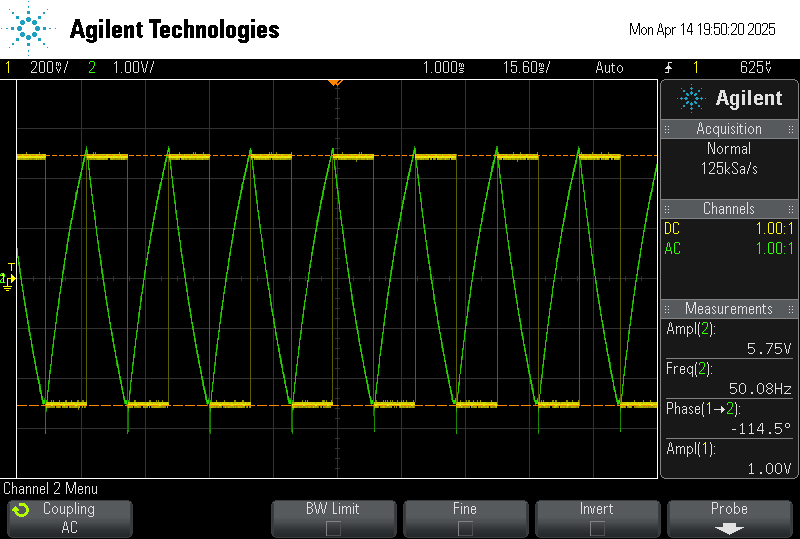
\includegraphics[width =0.85\textwidth]{figures/integrator_rechteck.png}
    \caption{Rechtecksignal und Integratorausgangssignal.}
    \label{fig:integrator_rechteck}
\end{figure}

\begin{figure}[h!]
    \centering
    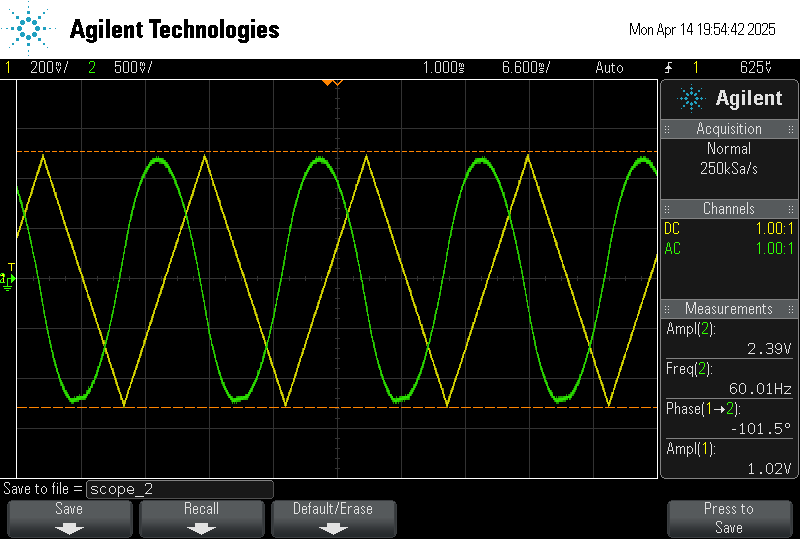
\includegraphics[width =0.85\textwidth]{figures/integrator_dreieck.png}
    \caption{Dreiecksignal und Integratorausgangssignal.}
    \label{fig:integrator_dreieck}
\end{figure}

\newpage

\subsection{Differenzierer}
\label{sec:Differenzierer_Auswertung}

Der Differenzierer wurde gemäß \autoref{fig:differenzierer} aufgebaut.
Es wurde der Widerstand $R = \qty{100}{\kilo\ohm}$ und die Kapazität $C = \qty{22}{\nano\farad}$ verwendet, was eine Zeitkonstante \newline
$\tau = RC = \qty{2.20e-3}{\second}$ liefert.


Auch hier wurde das Bode-Diagramm aufgenommen. Der gemessene Verlauf zeigt das erwartete lineare Ansteigen der Verstärkung mit der Frequenz, 
wie es für einen idealen Differentiator charakteristisch ist.

Der Verlauf in \autoref{plt:differenzierer} zeigt das erwartete 
lineare ansteigen proportional zu $f$ eines idealen Differenzierers,
dabei ist $A_{0,\text{theorie}} = 2 \pi R C$.

\begin{figure}[h!]
    \centering
    \includegraphics[width=\textwidth]{differentiator.pdf}
    \caption{Bode-Diagramm des Differenzierers mit $A_0 * f$ in $\unit{dB}$ auf der y-Achse und $f$ auf der x-Achse.}
    \label{plt:differenzierer}
\end{figure}

Gemäß \autoref{eq:differenzierer} ist das Ausgangssignal eines Differenzierers proportional zur
Ableitung des Eingangssignals. In \autoref{fig:differenzierer_rechteck} und
\autoref{fig:differenzierer_dreieck} ist die Signalspannung jeweils in Gelb und das Ausgangssignal in
Grün dargestellt.
\newpage

\begin{figure}[h!]
    \centering
    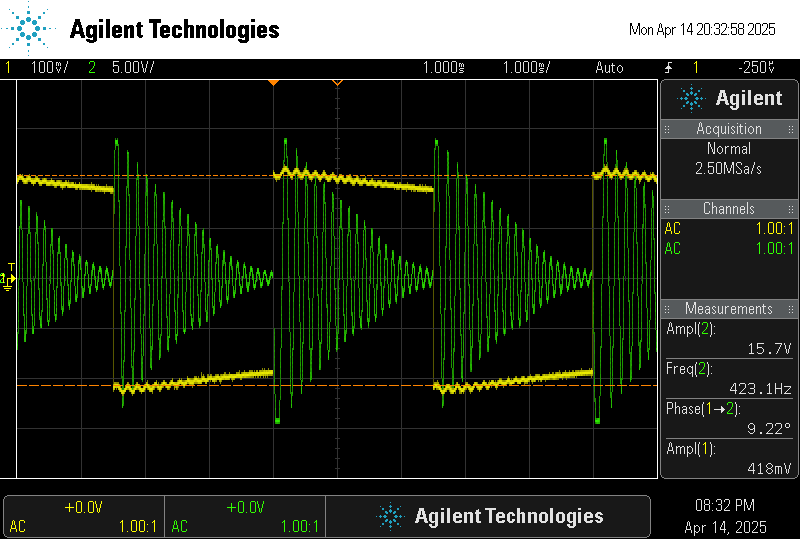
\includegraphics[width =0.85\textwidth]{figures/differenzierer_rechteck.png}
    \caption{Rechtecksignal und Differenziererausgangssignal.}
    \label{fig:differenzierer_rechteck}
\end{figure}

\begin{figure}[h!]
    \centering
    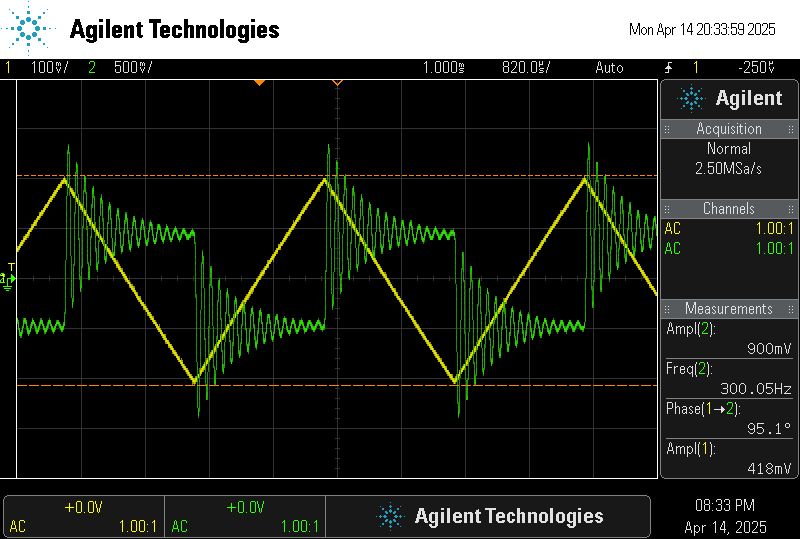
\includegraphics[width =0.85\textwidth]{figures/differenzierer_dreieck.png}
    \caption{Dreiecksignal und Differenziererausgangssignal.}
    \label{fig:differenzierer_dreieck}
\end{figure}

% Integrator messdaten
\begin{table}
    \centering
    \caption{Messdaten zum Integrator.}
    \label{tab:integrator}
    \resizebox{0.8\textwidth}{!}{%
    \begin{tblr}{
        colspec = {
            S[table-format=2.2]
            S[table-format=3.2]
            S[table-format=2.2]
            S[table-format=3.2]
            S[table-format=2.2]
            S[table-format=3.2]
        },
        row{1} = {guard},
        row{2} = {guard, mode = math}
    }
        \toprule
        \SetCell[c=2]{c} \textbf{Messpunkte 1-9} && \SetCell[c=2]{c} \textbf{Messpunkte 10-19} && \SetCell[c=2]{c} \textbf{Messpunkte 19-25} & \\
        \cmidrule[lr]{1-2} \cmidrule[lr]{3-4} \cmidrule[lr]{5-6}
        U_\text{out} \mathbin{/} \unit{\volt} & f \mathbin{/} \unit{\hertz} & 
        U_\text{out} \mathbin{/} \unit{\volt} & f \mathbin{/} \unit{\hertz} & 
        U_\text{out} \mathbin{/} \unit{\volt} & f \mathbin{/} \unit{\hertz} \\
        \midrule
            11.5 & 5  & 3.66 & 50  & 0.48          & 500           \\
            10.5 & 10 & 3.14 & 60  & 0.43          & 600           \\
            8.8  & 15 & 2.69 & 70  & 0.39          & 700           \\
            7.6  & 20 & 2.41 & 80  & 0.35          & 800           \\
            6.8  & 25 & 2.17 & 90  & 0.33          & 900           \\
            5.8  & 30 & 2.01 & 100 & 0.31          & 1000          \\
            5.2  & 35 & 1.04 & 200 & 0.31          & 2000          \\
            4.8  & 40 & 0.74 & 300 & $\mathbin{/}$ & $\mathbin{/}$ \\
            3.98 & 45 & 0.58 & 400 & $\mathbin{/}$ & $\mathbin{/}$ \\
        \bottomrule        	
    \end{tblr}
    }
\end{table}

% Differenzierer Messdaten
\begin{table}
    \centering
    \caption{Messdaten zum Differenzierer.}
    \label{tab:Differenzierer}
    \resizebox{0.8\textwidth}{!}{%
    \begin{tblr}{
        colspec = {
            S[table-format=2.2]
            S[table-format=3.2]
            S[table-format=2.2]
            S[table-format=3.2]
            S[table-format=2.2]
            S[table-format=3.2]
        },
        row{1} = {guard},
        row{2} = {guard, mode = math}
    }
        \toprule
        \SetCell[c=2]{c} \textbf{Messpunkte 1-5} && \SetCell[c=2]{c} \textbf{Messpunkte 6-10} && \SetCell[c=2]{c} \textbf{Messpunkte 11-15} & \\
        \cmidrule[lr]{1-2} \cmidrule[lr]{3-4} \cmidrule[lr]{5-6}
        U_\text{out} \mathbin{/} \unit{\volt} & f \mathbin{/} \unit{\kilo\hertz} & 
        U_\text{out} \mathbin{/} \unit{\volt} & f \mathbin{/} \unit{\kilo\hertz} & 
        U_\text{out} \mathbin{/} \unit{\volt} & f \mathbin{/} \unit{\kilo\hertz} \\
        \midrule
            0.065 & 0.03 & 0.370 & 0.30 & 0.960 & 0.80 \\
            0.087 & 0.05 & 0.490 & 0.40 & 1.090 & 0.90 \\
            0.115 & 0.07 & 0.600 & 0.50 & 1.190 & 1.00 \\
            0.145 & 0.10 & 0.740 & 0.60 & 2.390 & 2.00 \\
            0.257 & 0.20 & 0.840 & 0.70 & 3.680 & 3.00 \\
        \bottomrule        	
    \end{tblr}
    }
\end{table}

\subsection{Schmitt Trigger}
Aus \autoref{eq:SchmittTriggerSchaltschwelle} und den Komponenteneigenschaften aus \autoref{subsec:SchmittTrigger} 
kann der theoretische Wert berechnet $T_\text{theo} = \qty{29.89}{\volt}$ und mit dem experimentellen Wert $T_\text{exp}~=~\qty{28.1}{\volt}$
verglichen werden, woraus eine Abweichung von $\qty{6.00}{\percent}$ folgt. 

\subsection{Generator}
Der Theoretische Wert der Frequenz, welcher aus \autoref{eq:GeneratorFrequenz} berechnet wird, beträgt $f_\text{theo} = \qty{2.5}{\kilo\hertz}$.
Der Experimentelle Wert von $f_\text{exp} = \qty{1.67}{\kilo\hertz}$ weicht um $\qty{33.2}{\percent}$ vom Theorie Wert ab.

\subsection{Generator mit variierender Amplitude}
\label{sec:Generator_Auswertung}
Der Generator mit variierender Amplitude wurde gemäß \autoref{fig:generator} 
aufgebaut. Dabei wurden die Widerstände $R = \qty{10}{\kilo\ohm}$ und $R_1 = \qty{10}{\kilo\ohm}$ und für den Kondensatoren 
eine Kapazität $C = \qty{100}{\nano\farad}$.
Mittels eines Rechtecksignals wurden die Schwingungen des Generators angeregt. In \autoref{fig:generator_1} ist die Messung
der Schwingungen dargestellt. Dabei ist die Rechteckspannung in Gelb und die Ausgangsspannung in Grün dargestellt.

\begin{figure}
    \centering
    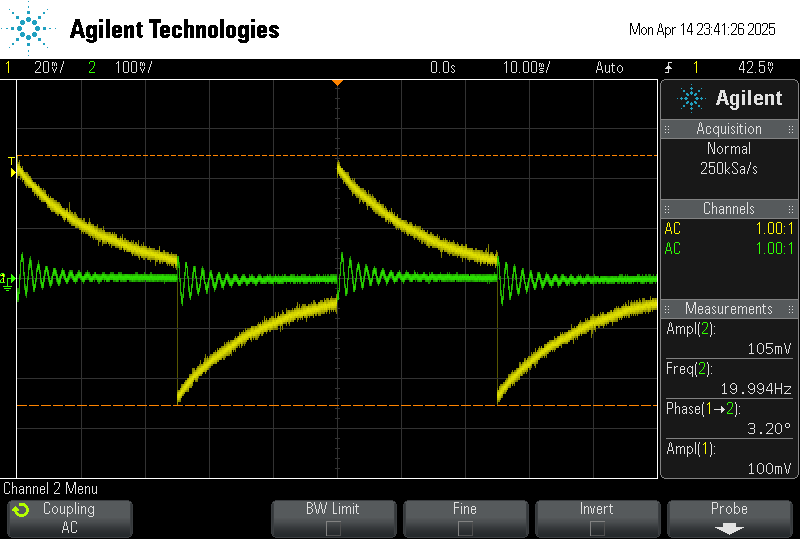
\includegraphics[width =\textwidth]{figures/scope_10.png}
    \caption{Angeregte Schwingungen am Generator mit variierender Amplitude.}
    \label{fig:generator_1}
\end{figure}

Gemäß \autoref{eq:GeneratorMitVariierenderAmplitudeLoesung} erwartet man einen exponentiellen
Abfall der Amplitude mit der Zeit. Dies kann durch den Zusammenhang

\begin{equation*}
    A(t) = A_0 \, \exp(-\frac{t}{\tau})
\end{equation*}

modelliert werden. Durch das logarithmieren dieser Gleichung ergibt sich die Geradengleichung

\begin{equation*}
    \ln(A(t)) = \ln(A_0) - \frac{t}{\tau}.
\end{equation*}

Es wird nun eine lineare Regression auf die logarithmierten Werte der Amplitude durchgeführt.
Die Amplitudenwerte werden für eine Anregung in \autoref{fig:generator_1}
abgelesen und in \autoref{tab:generator_1} aufgelistet.

\begin{table}
    \centering
    \caption{Zeitlicher Verlauf der Amplitude am Generator mit variierender Amplitude.}
    \label{tab:generator_1}
    \sisetup{table-format = 2.2} 
    \begin{tblr}{
        colspec = {S S S S S S},
        row{1} = {guard, mode = math}
    }
        \toprule 
        t \mathbin{/} \unit{\milli\second} & A \mathbin{/} \unit{\milli\volt} & \ln(U) &
        t \mathbin{/} \unit{\milli\second} & A \mathbin{/} \unit{\milli\volt} & \ln(U)  \\
        \midrule
        0.10  & 51.04 & -2.98 & 12.85 & 34.26 & -3.37 \\
        0.70  & 58.10 & -2.85 & 13.50 & 34.03 & -3.38 \\
        1.45  & 47.42 & -3.05 & 14.10 & 34.96 & -3.35 \\
        1.95  & 52.02 & -2.96 & 14.75 & 30.01 & -3.51 \\
        2.70  & 47.78 & -3.04 & 15.35 & 33.81 & -3.39 \\
        3.25  & 52.58 & -2.95 & 15.95 & 29.66 & -3.52 \\
        3.85  & 46.32 & -3.07 & 16.60 & 32.60 & -3.42 \\
        4.50  & 50.97 & -2.98 & 17.30 & 30.72 & -3.48 \\
        5.20  & 46.17 & -3.08 & 17.90 & 29.48 & -3.52 \\
        5.85  & 46.14 & -3.08 & 18.50 & 26.75 & -3.62 \\
        6.50  & 43.76 & -3.13 & 19.20 & 32.50 & -3.43 \\
        7.05  & 43.18 & -3.14 & 19.80 & 25.24 & -3.68 \\
        7.80  & 37.53 & -3.28 & 20.45 & 30.19 & -3.50 \\
        8.30  & 42.88 & -3.15 & 21.10 & 25.94 & -3.65 \\
        9.00  & 41.44 & -3.18 & 21.75 & 29.43 & -3.53 \\
        9.60  & 38.15 & -3.27 & 22.40 & 23.63 & -3.75 \\
        10.30 & 36.67 & -3.31 & 22.95 & 24.21 & -3.72 \\
        10.85 & 36.39 & -3.31 & 23.70 & 21.92 & -3.82 \\
        11.55 & 35.92 & -3.33 & 24.20 & 26.12 & -3.65 \\
        12.20 & 38.05 & -3.27 & 24.90 & 20.41 & -3.89 \\
        \bottomrule
    \end{tblr}
\end{table}

Die lineare Regression auf die logarithmierten Werte ist in \autoref{plt:generator_1_regression} 
dargestellt und ergibt die Parameter

\begin{equation}
    \tau_{\text{exp}} = \qty{288(12)}{\milli\second} \quad \text{und} \quad \ln(A_0) = \num{-2.91(0.02)}.
\end{equation}

\begin{figure}
    \centering
    \includegraphics[width =\textwidth]{build/generator_tau.pdf}
    \caption{Lineare Regression auf die logarithmierten Werte der Amplitude am Generator mit variierender Amplitude.}
    \label{plt:generator_1_regression}
\end{figure}

Der theoretische Wert $\tau_{\text{theo}}$ wird mit \autoref{eq:generatorMitVariierenderAmplitude} 
unter der Annahme $\abs{\eta} = 1$ berechnet und beträgt

\begin{equation}
    \tau_{\text{theo}} = \qty{200}{\milli\second}.
\end{equation}